\documentclass{article}
\usepackage[margin=1in]{geometry}
\usepackage{amsmath,amsthm,amssymb}
\usepackage{bbm,enumerate,mathtools}
\usepackage{tikz,pgfplots}
\usepackage{chessboard}
\usepackage[hidelinks]{hyperref}
\usepackage{multicol} % Problem 35
\usepackage{xstring} % Difficulty command
\usetikzlibrary{shapes.geometric}

\newenvironment{question}{\begin{trivlist}\item[\textbf{Question.}]}{\end{trivlist}}
\newenvironment{note}{\begin{trivlist}\item[\textbf{Note.}]}{\end{trivlist}}
\newenvironment{references}{\begin{trivlist}\item[\textbf{References.}]}{\end{trivlist}}
\newenvironment{related}{\begin{trivlist}\item[\textbf{Related.}]\end{trivlist}\begin{enumerate}}{\end{enumerate}}

\newcommand\score[1]{
\pgfmathsetmacro\pgfxa{#1+1}
\tikzstyle{scorestars}=[
  star,
  star points=5,
  star point ratio=2.25,
  draw,
  inner sep=3pt,
  anchor=outer point 5
]
  \begin{tikzpicture}[baseline]
    \draw[opacity=0] (0,-0.5) rectangle (0,0.2); % Workaround for whitespace at the bottom.
    \foreach \i in {1,...,4} {
      \pgfmathparse{(\i<=#1?"yellow":"gray")}
      \edef\starcolor{\pgfmathresult}
      \draw (\i*4.5ex,0) node[name=star\i,scorestars,fill=\starcolor]  {};
    }
  \end{tikzpicture}
}

\newcommand{\difficulty}[1]{%
  \IfEqCase{#1}{%
      {1}{
        
\begin{tikzpicture}[scale=0.7, baseline=0.9mm]%
          \definecolor{slopegreen}{rgb}{0.0, 0.5, 0.0}%
          \fill[slopegreen] (0.5,0.5) circle (0.5);%
        \end{tikzpicture}%
      }%
      {2}{
        
\begin{tikzpicture}[scale=0.7, baseline=0.9mm]%
          \definecolor{slopeblue}{rgb}{0.0, 0.44, 1.00}
          \fill[slopeblue] (0,0) rectangle (1,1);%
        \end{tikzpicture}%
      }%
      {3}{
\begin{tikzpicture}[scale=0.7, baseline=0.9mm]\fill (0,0.5)--(0.5, 0)--(1,0.5)--(0.5,1)--cycle; \end{tikzpicture}}%
      {4}{
\begin{tikzpicture}[scale=0.7, baseline=0.9mm]\fill (0.25,0)--(0,0.5)--(0.25,1)--(0.5,0.5)--cycle; \fill (0.75,0)--(0.5,0.5)--(0.75,1)--(1,0.5)--cycle;\end{tikzpicture}}%
      % you can add more cases here as desired
  }[\PackageError{difficulty}{Undefined difficulty level: #1}{}]%
}%
\newcommand{\rating}[2]{\difficulty{#1}\\\score{#2}\\}


\begin{document}
\rating{1}{2}
OEIS sequence
\href{https://oeis.org/A169950}{A169950} counts $0$-$1$ polynomials, $f(x)$, by their
\textit{thickness}: the magnitude of the largest coefficient in the expansion of $f(x)^2$.
\begin{quote}
  Consider the $2^n$ monic polynomials $f(x)$ with coefficients $0$ or $1$ and degree $n$.
  Sequence gives triangle read by rows, in which $T(n,k)$ ($n \geq 0$) is the number of such polynomials of thickness $k$ ($1 \leq k \leq n+1$).
\end{quote}
On
\href{https://twitter.com/oeisTriangles/status/1384302498442215427}{April 19, 2021}
my Twitter bot
\href{https://twitter.com/oeisTriangles}{@OeisTriangles}
tweeted an image in which that the parity of this triangle resembled the
The Sierpi\'nski triangle, suggesting that there is a recursive structure in
terms of the above rows.

\begin{figure}[ht!]
  \centering
  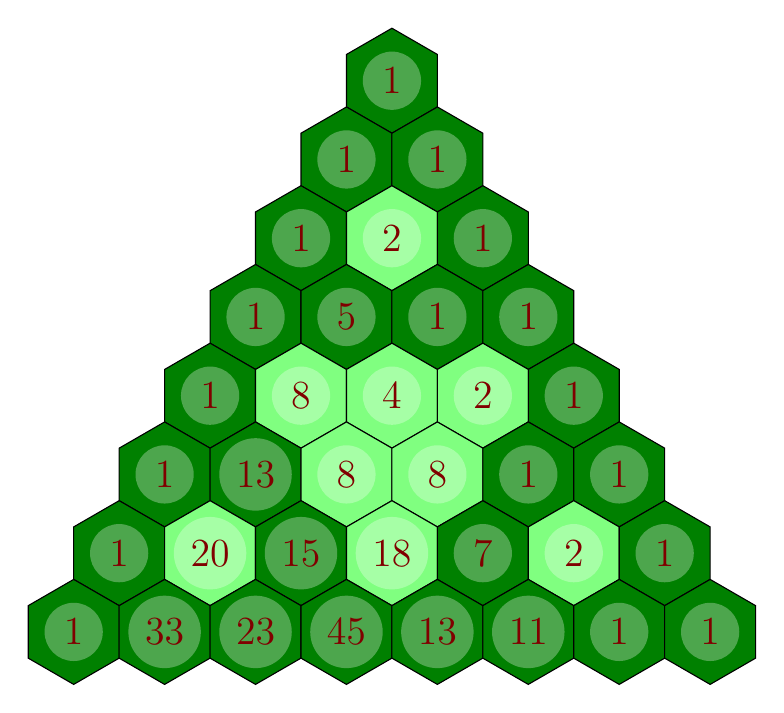
\begin{tikzpicture}
    \foreach \a/\b/\n/\c in {
      0/7/1/black,
      0/6/1/black, 1/6/1/black,
      0/5/1/black, 1/5/2/white, 2/5/1/black,
      0/4/1/black, 1/4/5/black, 2/4/1/black, 3/4/1/black,
      0/3/1/black, 1/3/8/white, 2/3/4/white, 3/3/2/white, 4/3/1/black,
      0/2/1/black, 1/2/13/black, 2/2/8/white, 3/2/8/white, 4/2/1/black, 5/2/1/black,
      0/1/1/black, 1/1/20/white, 2/1/15/black, 3/1/18/white, 4/1/7/black, 5/1/2/white, 6/1/1/black,
      0/0/1/black, 1/0/33/black, 2/0/23/black, 3/0/45/black, 4/0/13/black, 5/0/11/black, 6/0/1/black, 7/0/1/black}
    {
      \draw[
        fill=green!50!\c,
        xshift=\b*0.5774cm + \a*1.1547cm,
        yshift=\b cm
      ]
        (30:0.6667)--(90:0.6667)--(150:0.6667)--(210:0.6667)--(270:0.6667)--(330:0.6667)--cycle
      ;
      \node[
        circle,
        fill={white},
        fill opacity=0.3,
        text opacity=1,
        text=red!50!black,
        xshift=\b*0.5774cm + \a*1.1547cm,
        yshift=\b cm
      ] at (0,0) {\Large \n};
    }
  \end{tikzpicture}
  \caption{
    First eight rows of OEIS sequence A169950, where odd-valued cells are dark
    and even-valued cells are light.
  }
\end{figure}

\begin{question}
  What is a recurrence for the values in this triangle?
\end{question}

\begin{related}
  \item What if $\{-1,0,1\}$-polynomials are considered?
  \item What if the ``$m$-thickness'' is the largest coefficient when taken to
    the power $m$.
  \item What if the sum of coefficients is considered?
  \item How many $0$-$1$ polynomials $f(x)$ have $\operatorname{thickness}(f(x)) + 1 = \operatorname{thickness}(xf(x)+1)$?
    $\operatorname{thickness}(f(x)) + 2 = \operatorname{thickness}(xf(x)+1)$
    What is the asymptotic density of such $0$-$1$ polynomials as a function
    of degree?
\end{related}

\begin{references}
  \item \href{https://math.stackexchange.com/a/4176545/121988}{David Speyer, Math Stack Exchange answer}.
\end{references}
\end{document}
